\documentclass{article}
%--PASTE INTO MAIN FILE--
% \documentclass{article}
% %--PASTE INTO MAIN FILE--
% \documentclass{article}
% %--PASTE INTO MAIN FILE--
% \documentclass{article}
% \input{TexBase/DocumentBase.tex}
% \end{document}

\usepackage[margin = 0.7in]{geometry}
\usepackage{graphicx}
\usepackage{graphics}
\usepackage[T1]{fontenc}
\usepackage[polish]{babel}
\usepackage{cmap}
\usepackage[utf8]{inputenc}
\usepackage{float}
\usepackage{tabularx}
\usepackage[table,xcdraw]{xcolor}
\usepackage{lipsum}
\usepackage{titlesec}
\usepackage{minted}
\usepackage{xcolor}
\usepackage{caption}
\usepackage{enumitem}
\usepackage{csvsimple}
\usepackage{natbib}
\usepackage{blindtext}

\usepackage{amsmath} %math

\usepackage{numprint} % rounding
\usepackage[round-precision=3,round-mode=figures, scientific-notation=true]{siunitx} %scientific notation

\usepackage[hidelinks]{hyperref}
\usepackage{url}

\usepackage{bm} %bold for math


%TABS
\usepackage[]{booktabs}
\usepackage{tabularray}
\usepackage{multirow}

%\title{}
\author{Michał Dziedziak}
\date{\today}


\titlespacing\section{0pt}{12pt plus 4pt minus 2pt}{0pt plus 2pt minus 2pt}
\titlespacing\subsection{0pt}{12pt plus 4pt minus 2pt}{0pt plus 2pt minus 2pt}
\titlespacing\subsubsection{0pt}{12pt plus 4pt minus 2pt}{0pt plus 2pt minus 2pt}
\setlength{\parskip}{\baselineskip}%
\setlength{\parindent}{0pt}%

\newcommand{\squeezeup}{\vspace{-5mm}}


\begin{document}

\begin{titlepage}
    \begin{center}
        \vspace*{5cm}
        \rule{500pt}{1pt}\\
        \vspace*{0.5cm}
        \LARGE
        \textbf{Inżyniera Obrazów}\\
        \Large
        Laboratorium numer 2
        \vspace*{0.5cm}
        \rule{500pt}{1pt}
    \end{center}

    \vspace*{10cm}

    {\raggedright
        \large
        \textbf{Autor sprawozdania:} Michał Dziedziak 263901\\
        \textbf{Imię i Nazwisko prowadzącego kurs:} dr inż. Jan Nikodem\\
        \textbf{Dzień i godzina zajęć:} czwartek, 11:15 - 14:15
    }
\end{titlepage}


\tableofcontents
% \listoftables

%\renewcommand\listoflistingscaption{List of source codes}
% \listoflistings

\listoffigures


\newpage


% \begin{table}[H]
%     \centering
%     \begin{tabular}{|c|c|c|c|}%
%         \hline
%         \bfseries Numer iteracji & \bfseries Czas zalezienia rozwiązania [ms] & Koszt ścieżki & Błąd względny% specify table head
%         \csvreader[head to column names]{Csv/BestPathTest_SimulatedAnnealing_LINEAR_ftv47.csv}{}% use head of csv as column names
%         {\\\hline\Iteration & \num{\TimeInMiliSeconds} & \Cost & \num[round-precision=2, round-mode=places, scientific-notation=false]{\Error}\%}% specify your columns here
%         \\\hline    
%     \end{tabular}
%     \caption{}
%     \label{tab:}
% \end{table}

% \begin{figure}[H]
%     \centering
%     \resizebox{\columnwidth}{!}{%
%     \includegraphics{}%
%     }
%     \caption{}
%     \label{fig:}
% \end{figure}

% \begin{listing}[H]
%     \begin{minted}[frame=single,framesep=2mm,linenos,fontsize=\footnotesize]{language}
%         some code
%     \end{minted}
%     \caption{}
%     \label{lst:}
% \end{listing}


% \bibliographystyle{plainnat}
% \bibliography{TexBase/Bibliography}

% \end{document}

\usepackage[margin = 0.7in]{geometry}
\usepackage{graphicx}
\usepackage{graphics}
\usepackage[T1]{fontenc}
\usepackage[polish]{babel}
\usepackage{cmap}
\usepackage[utf8]{inputenc}
\usepackage{float}
\usepackage{tabularx}
\usepackage[table,xcdraw]{xcolor}
\usepackage{lipsum}
\usepackage{titlesec}
\usepackage{minted}
\usepackage{xcolor}
\usepackage{caption}
\usepackage{enumitem}
\usepackage{csvsimple}
\usepackage{natbib}
\usepackage{blindtext}

\usepackage{amsmath} %math

\usepackage{numprint} % rounding
\usepackage[round-precision=3,round-mode=figures, scientific-notation=true]{siunitx} %scientific notation

\usepackage[hidelinks]{hyperref}
\usepackage{url}

\usepackage{bm} %bold for math


%TABS
\usepackage[]{booktabs}
\usepackage{tabularray}
\usepackage{multirow}

%\title{}
\author{Michał Dziedziak}
\date{\today}


\titlespacing\section{0pt}{12pt plus 4pt minus 2pt}{0pt plus 2pt minus 2pt}
\titlespacing\subsection{0pt}{12pt plus 4pt minus 2pt}{0pt plus 2pt minus 2pt}
\titlespacing\subsubsection{0pt}{12pt plus 4pt minus 2pt}{0pt plus 2pt minus 2pt}
\setlength{\parskip}{\baselineskip}%
\setlength{\parindent}{0pt}%

\newcommand{\squeezeup}{\vspace{-5mm}}


\begin{document}

\begin{titlepage}
    \begin{center}
        \vspace*{5cm}
        \rule{500pt}{1pt}\\
        \vspace*{0.5cm}
        \LARGE
        \textbf{Inżyniera Obrazów}\\
        \Large
        Laboratorium numer 2
        \vspace*{0.5cm}
        \rule{500pt}{1pt}
    \end{center}

    \vspace*{10cm}

    {\raggedright
        \large
        \textbf{Autor sprawozdania:} Michał Dziedziak 263901\\
        \textbf{Imię i Nazwisko prowadzącego kurs:} dr inż. Jan Nikodem\\
        \textbf{Dzień i godzina zajęć:} czwartek, 11:15 - 14:15
    }
\end{titlepage}


\tableofcontents
% \listoftables

%\renewcommand\listoflistingscaption{List of source codes}
% \listoflistings

\listoffigures


\newpage


% \begin{table}[H]
%     \centering
%     \begin{tabular}{|c|c|c|c|}%
%         \hline
%         \bfseries Numer iteracji & \bfseries Czas zalezienia rozwiązania [ms] & Koszt ścieżki & Błąd względny% specify table head
%         \csvreader[head to column names]{Csv/BestPathTest_SimulatedAnnealing_LINEAR_ftv47.csv}{}% use head of csv as column names
%         {\\\hline\Iteration & \num{\TimeInMiliSeconds} & \Cost & \num[round-precision=2, round-mode=places, scientific-notation=false]{\Error}\%}% specify your columns here
%         \\\hline    
%     \end{tabular}
%     \caption{}
%     \label{tab:}
% \end{table}

% \begin{figure}[H]
%     \centering
%     \resizebox{\columnwidth}{!}{%
%     \includegraphics{}%
%     }
%     \caption{}
%     \label{fig:}
% \end{figure}

% \begin{listing}[H]
%     \begin{minted}[frame=single,framesep=2mm,linenos,fontsize=\footnotesize]{language}
%         some code
%     \end{minted}
%     \caption{}
%     \label{lst:}
% \end{listing}


% \bibliographystyle{plainnat}
% \bibliography{TexBase/Bibliography}

% \end{document}

\usepackage[margin = 0.7in]{geometry}
\usepackage{graphicx}
\usepackage{graphics}
\usepackage[T1]{fontenc}
\usepackage[polish]{babel}
\usepackage{cmap}
\usepackage[utf8]{inputenc}
\usepackage{float}
\usepackage{tabularx}
\usepackage[table,xcdraw]{xcolor}
\usepackage{lipsum}
\usepackage{titlesec}
\usepackage{minted}
\usepackage{xcolor}
\usepackage{caption}
\usepackage{enumitem}
\usepackage{csvsimple}
\usepackage{natbib}
\usepackage{blindtext}

\usepackage{amsmath} %math

\usepackage{numprint} % rounding
\usepackage[round-precision=3,round-mode=figures, scientific-notation=true]{siunitx} %scientific notation

\usepackage[hidelinks]{hyperref}
\usepackage{url}

\usepackage{bm} %bold for math


%TABS
\usepackage[]{booktabs}
\usepackage{tabularray}
\usepackage{multirow}

%\title{}
\author{Michał Dziedziak}
\date{\today}


\titlespacing\section{0pt}{12pt plus 4pt minus 2pt}{0pt plus 2pt minus 2pt}
\titlespacing\subsection{0pt}{12pt plus 4pt minus 2pt}{0pt plus 2pt minus 2pt}
\titlespacing\subsubsection{0pt}{12pt plus 4pt minus 2pt}{0pt plus 2pt minus 2pt}
\setlength{\parskip}{\baselineskip}%
\setlength{\parindent}{0pt}%

\newcommand{\squeezeup}{\vspace{-5mm}}


\begin{document}

\begin{titlepage}
    \begin{center}
        \vspace*{5cm}
        \rule{500pt}{1pt}\\
        \vspace*{0.5cm}
        \LARGE
        \textbf{Inżyniera Obrazów}\\
        \Large
        Laboratorium numer 2
        \vspace*{0.5cm}
        \rule{500pt}{1pt}
    \end{center}

    \vspace*{10cm}

    {\raggedright
        \large
        \textbf{Autor sprawozdania:} Michał Dziedziak 263901\\
        \textbf{Imię i Nazwisko prowadzącego kurs:} dr inż. Jan Nikodem\\
        \textbf{Dzień i godzina zajęć:} czwartek, 11:15 - 14:15
    }
\end{titlepage}


\tableofcontents
% \listoftables

%\renewcommand\listoflistingscaption{List of source codes}
% \listoflistings

\listoffigures


\newpage


% \begin{table}[H]
%     \centering
%     \begin{tabular}{|c|c|c|c|}%
%         \hline
%         \bfseries Numer iteracji & \bfseries Czas zalezienia rozwiązania [ms] & Koszt ścieżki & Błąd względny% specify table head
%         \csvreader[head to column names]{Csv/BestPathTest_SimulatedAnnealing_LINEAR_ftv47.csv}{}% use head of csv as column names
%         {\\\hline\Iteration & \num{\TimeInMiliSeconds} & \Cost & \num[round-precision=2, round-mode=places, scientific-notation=false]{\Error}\%}% specify your columns here
%         \\\hline    
%     \end{tabular}
%     \caption{}
%     \label{tab:}
% \end{table}

% \begin{figure}[H]
%     \centering
%     \resizebox{\columnwidth}{!}{%
%     \includegraphics{}%
%     }
%     \caption{}
%     \label{fig:}
% \end{figure}

% \begin{listing}[H]
%     \begin{minted}[frame=single,framesep=2mm,linenos,fontsize=\footnotesize]{language}
%         some code
%     \end{minted}
%     \caption{}
%     \label{lst:}
% \end{listing}


% \bibliographystyle{plainnat}
% \bibliography{TexBase/Bibliography}



\section{Temat laboratorium}
W ramach trzecich zajęć laboratoryjnych mieliśmy wykonać zadanie 4 i 5 z listy drugiej.
Punkty te dotyczyły implementacji algorytmu JPEG.


\section{Zadania do wykonania i plan pracy}

\subsection{Zadanie 4: Implementacja części algorytmu JPEG}
Zadanie czwarte zakładało uproszczoną implementację algorytmu JPEG. W ramach tego punktu mieliśmy
zaimplementować:
\begin{itemize}
    \item Kroki: 0, 1, 2, 3, 7, 8 algorytmu JPEG. Gdzie:
          \begin{itemize}
              \item Krok 0: Wczytanie obrazu wejściowego,
              \item Krok 1: Konwersja modelu barw: RGB -> YCbCr,
              \item Krok 2: Przeskalowanie w dół macierzy składowych Cb i Cr,
              \item Krok 3: Podział na bloki o rozmiarze 8x8,
              \item Krok 7: Zwinięcie każdego bloku 8x8 do wiersza 1x64 - algorytm ZigZag,
              \item Krok 8: Zakodowanie danych obrazu,
          \end{itemize}
    \item Zmierzyć liczbę bajtów powstałego obrazu po kroku 8
    \item Ocenić wpływ kroku 2. na rozmiar i wygląd, poprzez stworzenie trzech wariancji obrazu:
          \begin{itemize}
              \item bez próbkowania,
              \item z próbkowaniem ci drugi element,
              \item z próbkowaniem co czwarty element.
          \end{itemize}
    \item Dokonać dekompresji poprzez odwrócenie powyższych kroków.
\end{itemize}

\subsection{Zadanie 5: Dokończenie implementacji algorytmu JPEG}
Zadanie piąte zakładało dokończenie implementacji algorytmu JPEG. W ramach tego punktu mieliśmy
zaimplementować:
\begin{itemize}
    \item Pozostałe kroki algorytmu:
          \begin{itemize}
              \item Krok 4: Wykonanie dyskretnej transformacji cosinusowej na każdym bloku obrazu,
              \item Krok 5: Podzielenie każdego bloku obrazu przez macierz kwantyzacji,
              \item Krok 6: Zaokrąglenie wartości w każdym bloku do liczb całkowitych.
          \end{itemize}
    \item Ocenić jak wybór czynnika QF wpływa na rozmiar i wygląd obrazka.
    \item Dokonać dekompresji poprzez odwrócenie powyższych kroków.
\end{itemize}

\section{Teoria}

Format JPEG (ang. Joint Photographic Experts Group) jest powszechnie stosowanym standardem kompresji
stratnej do obrazów cyfrowych. Algorytm JPEG składa się z kilku etapów, które pozwalają na efektywną
redukcję rozmiaru pliku przy minimalnej utracie jakości obrazu.

\subsection{Konwersja modelu barw: RGB -> YCbCr}
W pierwszym kroku obraz jest konwertowany z modelu barw RGB do przestrzeni barw YCbCr. Model YCbCr składa
się z trzech składowych: Y (luminancja), Cb (chrominancja niebieska) i Cr (chrominancja czerwona).
Konwersja ta pozwala na oddzielenie informacji o jasności od informacji o barwie, co ułatwia dalszą kompresję.

\subsection{Przeskalowanie w dół macierzy składowych Cb i Cr}
Kolejnym krokiem jest przeskalowanie macierzy składowych Cb i Cr, które odpowiadają za informacje o barwie,
przy użyciu technik próbkowania, takich jak próbkowanie co drugi element lub co czwarty element.
To przeskalowanie pozwala na zmniejszenie rozmiaru danych przy minimalnej utracie jakości obrazu.

\subsection{Podział obrazu na bloki o rozmiarze 8x8}
Obraz jest dzielony na niewielkie bloki o stałym rozmiarze 8 na 8 pikseli. Ten krok umożliwia stosowanie
transformacji i kwantyzacji na mniejszych fragmentach obrazu, co ułatwia kompresję.

\subsection{Wykonanie dyskretnej transformacji cosinusowej (DCT)} %TODO to lepiej opisać
Każdy blok obrazu jest poddawany dyskretnej transformacji cosinusowej (DCT), która przekształca blok
pikseli z dziedziny przestrzennej do dziedziny częstotliwości. DCT pozwala na koncentrację energii
sygnału obrazu w niewielkiej liczbie współczynników, co ułatwia kwantyzację.

\subsection{Podzielenie każdego bloku obrazu przez macierz kwantyzacji} %TODO to lepiej opisać
Wyniki DCT są dzielone przez macierz kwantyzacji, która zawiera współczynniki kwantyzacji dla różnych
częstotliwości.
Wysokie wartości w macierzy kwantyzacji prowadzą do większej utraty informacji i większej kompresji.

\subsection{Zaokrąglenie wartości w każdym bloku do liczb całkowitych}
Po podzieleniu przez macierz kwantyzacji wartości wynikowe są zaokrąglane do najbliższych liczb całkowitych,
co dodatkowo redukuje rozmiar danych.

\subsection{Zwinięcie każdego bloku 8x8 do wiersza 1x64 - algorytm ZigZag}
W celu dalszej kompresji, współczynniki kwantyzacji są uporządkowywane za pomocą
algorytmu ZigZag, który umożliwia efektywne kodowanie długich sekwencji zer.

\subsection{Zakodowanie danych obrazu – m.in. algorytmem Huffmana} %TODO Opisać algorytm Huffmana i upewnić się że go używam
Ostatecznie, dane obrazu są kodowane za pomocą różnych algorytmów kompresji, takich
jak algorytm Huffmana, który redukuje redundancję danych i dalszy zmniejsza rozmiar pliku.

Algorytm JPEG umożliwia osiągnięcie znacznej kompresji obrazu przy zachowaniu akceptowalnej jakości wizualnej.
Parametry takie jak czynnik jakości (Quality Factor) pozwalają na regulację kompromisu pomiędzy
jakością obrazu a stopniem kompresji.


% TODO Więcej źródeł
Źródła: \cite{Fileformat}

\section{Prezentacja wykonanego zadania}

\begin{figure}[H]
    \centering
    \resizebox{\columnwidth}{!}{%
        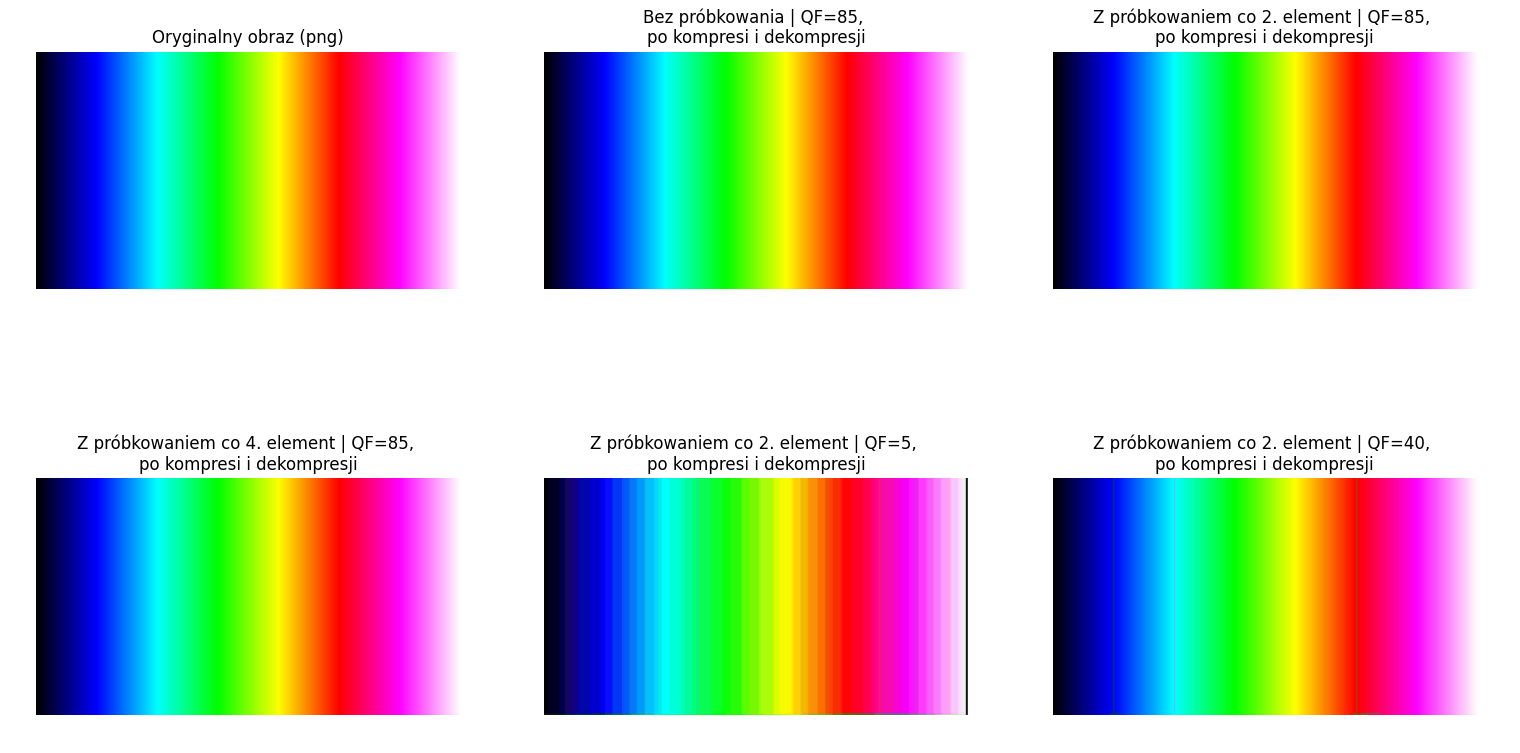
\includegraphics{Img/zad45.png}%
    }
    \caption{Prezentacja oryginalnego obrazu wraz z wariacjami po kompresji i dekompresji (z różnymi parametrami)}
    \label{fig:zad45}
\end{figure}


\begin{figure}[H]
    \centering
    \resizebox{\columnwidth / 2}{!}{%
        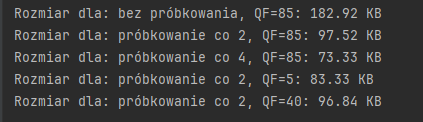
\includegraphics{Img/zad45_1.png}%
    }
    \caption{Logi konsoli opisujące rozmiary obrazów po kompresji (z różnymi parametrami)}
    \label{fig:zad45_1}
\end{figure}

\section{Wnioski}
Podczas laboratorium pomyślnie zaimplementowałem algorytm JPEG.
Udało mi się zrozumieć poszczególne kroki algorytmu i ich wpływ na rozmiar i jakość obrazu.
Na podstawie wykonanych zadań zauważyłem, że wybór parametrów takich jak czynnik jakości (QF) czy technika
próbkowania ma znaczący wpływ na rozmiar i jakość obrazu.
\begin{itemize}
    \item Wraz ze wzrostem czynnika jakości (QF) rośnie jakość obrazu, ale maleje stopień kompresji (co za tym
          idzie, zwiększa się rozmiar obrazu).
    \item Technika próbkowania również wpływa na rozmiar obrazu. Wraz ze wzrostem stopnia próbkowania
          maleje rozmiar obrazu, ale rośnie utrata jakości.
\end{itemize}

\bibliographystyle{plainnat}
\bibliography{TexBase/Bibliography}

\end{document}